\documentclass[../ZF_Wing.tex]{subfiles}
\begin{document}

\subsection{Materialwirtschaft}
\colorbox{blue!30}{\textbf{Materialbewegung:}}
\begin{itemize}
	\item Verwaltung
	\item Planung
	\item Steuerung
	
\end{itemize}
\colorbox{blue!30}{\textbf{2 Aufgaben:}}
\begin{enumerate}
	\item Technische Aufgabe
	\item Wirtschaftliche Aufgabe

\end{enumerate}
\colorbox{blue!30}{\textbf{Bestandteile:}}
\begin{itemize}
	\item Beschaffungslogistik
	\begin{itemize}
		\item Bedarfsermittlung
		\item Beschaffungsmarktforschung
	\end{itemize}
	\item Produktionslogistik
	\begin{itemize}
		\item Verbrauchsermittlung
		\item Produktionsplanung
	\end{itemize}
	\item Lagerlogistik
	\begin{itemize}
		\item Lagerung
		\item Bestandesermittlung
	\end{itemize}
	\item Absatzlogistik
	\begin{itemize}
		\item Distribution
	\end{itemize}
	\item Entsorgungslogistik
	\begin{itemize}
		\item Entsorgung
	\end{itemize}
\end{itemize}


\begin{figure}[H]
\centering
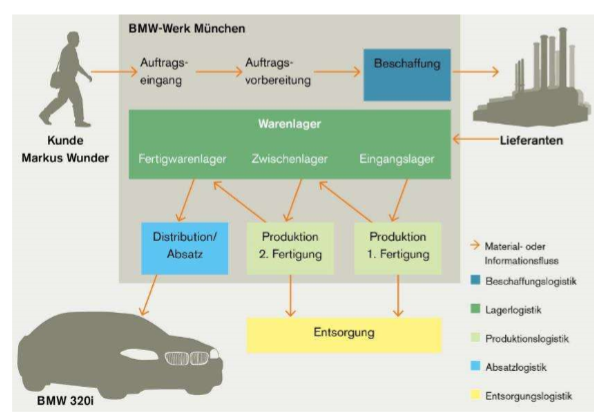
\includegraphics[width=0.3\textwidth]{Resources/Image/Logistik.png}
\caption{\label{fig:GliederungER}Logistik.}
\end{figure}


\subsubsection{Beschaffungslogistik}
\colorbox{green!30}{\textbf{Beschaffungsprozesse}}

\begin{enumerate}
	\item Ermittlung Materialbedarf für Produktion
	\item Ermittlung Lagerbestände
	\item Ermittlung Beschaffungsbedarf
	\item Lieferantenwahl
	\item Bestellungen
	\item Wareneingangskontrolle
\end{enumerate}
\colorbox{green!30}{\textbf{Beschaffungsobjekte}}
\begin{itemize}
	\item Rohstoffe
	\item Hilfsstoffe
	\item Beriebsstoffe
	\item Montageteile
	\item Handelswaren
\end{itemize}
\colorbox{green!30}{\textbf{Beschaffungsobjekte}}
\begin{itemize}
	\item Vorratsbeschaffung (Order to stock)
	\item Fallweise Beschaffung (order to make)
	\begin{itemize}
		\item Lagerhaltung an Lieferanten übertragen
	\end{itemize}
	\item Just in Time
	\begin{itemize}
		\item Auch Lieferant beginnt erst mit Fertigung, wenn Kundenauftrag vorliegt
		\item funktioniert nur wenn auf pünktliche Lieferung verttraut werden kann.
	\end{itemize}
	\item Just in Sequence
\end{itemize}

\subsubsection{Insourcing}
Verlagerung von zuvor im Markt bezogenen Leistungen in die eigene Wertschöpfung.\\\\
\textbf{Vorteile:}
\begin{itemize}
	\item Reduktion Lieferzeiten
	\item Unabhängigkeit von Lieferanten, Preisen und Absatzmengen
	\item Aufrechterhaltung Qualitätsstandards
	\item Auslastung Fertigungskapazitäten
\end{itemize}

\subsubsection{Outsourcing}
Verlagerung von Teilen der Wertschöpfung auf externe Lieferanten (langfristig).\\\\
\textbf{Vorteile:}
\begin{itemize}
	\item Minimierung der Fixkosten
	\item Beschaffungsmenge und Zeitspanne flexibel planbar
	\item Minimierung der Lagerkosten
	\item Ausweichmöglichkeit bei Kapazitätsengpässen
\end{itemize}

\subsubsection{Entscheid Make or buy}

Kostenfunktion ``make'' : \colorbox {teal!30} {K = Variable Kosten pro Stück + Fixkosten}\\
Kostenfunktion ``buy''  : \colorbox {teal!30} {K = Variable Kosten pro Stück}\\
Kostenfunktion ``make'' = Kostenfunktion ``buy''
Variable Kosten pro Stk. * x + Fixkosten = Variable Kosten pro Stück * x\\\\
\textbf{Vorteile Buy:}
\begin{itemize}
	\item Konzentration auf Kerngeschäft
	\item Zugang zu Know-how (vom Zulieferer)
	\item Freisetzung von Kapazitäten und Finanzmittel
	\item Bessere Steuerbarkeit der Kosten
	\item Standardisierung und klar definierte Leistungen
\end{itemize}
\textbf{Nachteile Buy:}
\begin{itemize}
	\item Abhängigkeit
	\item Risiko schlechte Leistung des Outsourcing Partners
	\item Langfristiger Verlust von Know-how
	\item Sensible Daten, Geheimhaltung
	\item Schwer rückgängig zu machen
	\item Transaktions- und Umsetzungskosten
	\item Kommunikationsintensiv (Informatiosdefiziten)
\end{itemize}


\subsection{Magisches Dreieck der Materialwirtschaft}
\begin{itemize}
	\item Kapitalbindung und Lagerunterhalt
	\item Beschaffungskosten
	\item Lieferbereitschaft

\end{itemize}

\subsubsection{ABC-Analyse I}
\begin{itemize}
	\item Menge der gelagerten Teile samt Einstandspreis auflisten
	\item Lagerwert = Menge *  Einstandspreis/Stk.
	\item Identifizieren: Welche Beschaffungsobjekte wertvoll sind und damit viel Kapital binden
\end{itemize}

\subsubsection{ABC-Analyse II}
Unterteilung der Produkte in A,B,C (ganz teuere, ganz günstige).\\
Anwendungsmöglichkeiten:
\begin{itemize}
	\item Kostenarten : Kostenvolumen
	\item Optimierung
	\item Key-Account-Management (Umsatzanteil von Lieferanten-/Kundengruppen)
\end{itemize}
x-Achse Menge in $\%$\\
y-Achse Lagerwert in $\%$\\


\subsubsection{ABC-Analyse III}
\colorbox {red!30}{A-Güter:}
\begin{itemize}
	\item 70-80\% Wertanteil des Gesamtwerts
	\item $<$30 \% Mengenanteil der Gesamtmenge
\end{itemize}
\colorbox {red!30}{B-Güter:}
\begin{itemize}
	\item 15-20\% Wertanteil des Gesamtwerts
	\item 30-50 \% Mengenanteil der Gesamtmenge
\end{itemize}
\colorbox {red!30}{C-Güter:}
\begin{itemize}
	\item 5-10\% Wertanteil des Gesamtwerts
	\item 40-50 \% Mengenanteil der Gesamtmenge
\end{itemize}
\textbf{Lagerwertreduzierung:} Konzentration der Planungs- und Organisationsarbeiten auf A-Güter.\\
\textbf{Senkung Lagerunterhaltskosten:} Minimierung voluminöser Güter\\

\subsection{XYZ-Analyse}
\textcolor {blue} {X-Güter:} Regelmässiger Bedarf / Vorhersagegenuigkeit ist hoch.\\\textcolor {blue} {Y-Güter:} Schwankender Bedarf / Vorhersagegenuigkeit ist begrenzt.\\
\textcolor {blue} {Z-Güter:} Unregelmässiger Bedarf / Vorhersagegenuigkeit ist gering.\\

\begin{itemize}
	\item Ergänzung zur ABC-Analyse
	\item Einteilung in Güterkategorien aufgrund Vorhersagegenauigkeit des Bedarfs
	\item X-Güter: Kontinuierlicher Materialfluss möglich
	\item Y- und Z-Güter: Bedarfsschwankungen, welche durch die Lagerbestände aufgefangen werden können
\end{itemize}

\subsection{Lagerorganisation}
\begin{itemize}
	\item Eingangslager: Vor der Produktion, versorgen Produktion mit nötigen Materialien
	\item Zwischenlager: Paraallel zur Produktion
	\item Fertigwarenlager: Fertigprodukte und Handelswaren
\end{itemize}

\subsubsection{Lagerfunktionen I}
\begin{itemize}
	\item Zeitüberbrückung
	\item Sicherung
	\item Spekulation
\end{itemize}

\subsubsection{Lagerfunktionen II}
\begin{itemize}
	\item Veredelung bzw. Umformung
	\item Assortierung
\end{itemize}

\subsection{Kennzahlen der Lagerhaltung}

Durchsch. Lagerbestand $= \dfrac{Anfangsbestand + Endbestand}{2}$\\\\
Lagerumschlagshäufigkeit (Je höher, desto niedriger das im Lager gebundene Kapital) $= \dfrac{Jahresverbrauch}{Durchsch. Lagerbestand}$\\\\
Durchschnittliche Lagerdauer(Je kürzer, desto geringer Kaptialbindungsdauer) $= \dfrac{360}{Umschlagshaeufigkeit}$\\
























































\end{document}